% !TEX encoding = UTF-8
% !TEX TS-program = pdflatex
% !TEX root = ../tesi.tex
% !TEX spellcheck = it-IT

%************************************************
\chapter{Classificazione}
\label{cap:ctbnc}
%************************************************
La classificazione è un argomento centrale nei campi di ricerca relativi all'\keyword{apprendimento automatico} (anche detto \keyword{machine learning}) e l'analisi dei dati. In generale, essa consiste nel processo di assegnare una \emph{classe} (\ie{} un'etichetta) a delle istanze descritte da un insieme di attributi. Si parla di \emph{classificazione \keywordsub[classificazione]{supervisionata}} quando è necessario indurre un \keywordsub[classificazione]{classificatore} a partire da un insieme di dati composto da istanze già etichettate e utilizzare tale classificatore per classificare nuove istanze di dati.

In questo capitolo viene quindi introdotta una classe di modelli, che prende il nome di \acf{CTBNC}, il cui scopo è la \emph{classificazione supervisionata} di traiettorie multivariate di variabili discrete a \emph{tempo continuo}. Si descrivono due istanze di tale classe: i classificatori \acf{CTNB} e i classificatori \acf{CTTANB}; classificatori per i quali si affronta il processo di apprendimento in caso di dati completi (\autoref{sec:learning-ctbnc}).

Infine, nella \autoref{sec:inference-ctbnc}, si presenta un algoritmo di inferenza esatta per la classe dei \acs{CTBNC}.

\section{Modello}\label{sec:ctbnc-model}
Al fine di risolvere il succitato problema della classificazione sono stati proposti numerosi approcci. Ad esempio \lwcase \nb{} \class{}, un classificatore semplice ma robusto proposto da~\citet{DudaHart1973}; rivelatosi essere uno fra i classificatori più performanti~\citep{Langley1992}. Esso apprende dai dati la probabilità condizionale di ogni attributo $\setel{A}_i$ data la classe $\setel{C}$. La classificazione di nuove istanze dei dati è effettuata applicando la \emph{regola di Bayes} al fine di calcolare la probabilità della classe $\setel{C}$ data l'istanziazione di $\setel{A}_i,\,\dotsc\,,\setel{A}_N$ e scegliendo quella con la maggiore probabilità a posteriori. Questo calcolo è reso possibile da un'assunzione forte: tutti gli attributi $\setel{A}_i$ sono \emph{condizionalmente indipendenti} (\myref[si veda la definizione]{defn:ic}) tra di loro data evidenza sulla classe $\setel{C}$.

Poiché tale assunzione è chiaramente irreale,~\citet{Friedman1997} ha investigato come migliorare ulteriormente le prestazioni del \lwcase \nb{} \class{} evitando assunzioni di indipendenza non giustificate dai dati. A tal fine~\citet{Friedman1997}, generalizzando il \lwcase \nb{} \class{}, ha proposto una classe di modelli di \emph{classificazione supervisionata}, chiamata \acf{BNC} (di cui fa parte il \acf{TAN} \class{}, ad esempio) che ereditano dalla teoria delle \acl{BN} (\myref[si rimanda alla definizione]{defn:bn} per maggiori dettagli) una rappresentazione fattorizzata delle distribuzioni di probabilità dei nodi attributo e rappresentano esplicitamente le indipendenze condizionali fra essi.

Seguendo le stesse motivazioni, in ~\citet{Stella2012} viene formalizzata una classe di modelli di \emph{classificazione supervisionata}, chiamati \acf{CTBNC}, derivata dalle \acs{CTBN} (\myref[si veda la definizione]{defn:ctbn}).

Di seguito si definiscono quindi i \acl{CTBNC} e due istanze di classificatori appartenenti a tale classe: il \acf{CTNBC} e il \acf{CTTANBC}.

Un \acl{CTBNC} estende una \acs{CTBN} tramite l'aggiunta di un nodo associato alla variabile classe $\setel{Y}$. Si ricorda, dalla \myref[definizione]{defn:ctbn}, che una \acs{CTBN} rappresenta l'evoluzione nel tempo continuo di una variabile di processo $\set{X}$ (\ie{} insieme composto da $N$ \mprocess{}, \myref[si veda la definizione]{defn:pv}).

Di seguito si dà la definizione di questa nuova classe di modelli di \emph{classificazione supervisionata}.
\begin{definizione}[\acl{CTBNC}]\label{defn:ctbnc}
Un \acf{CTBNC} è composto da una coppia $\conceptsym{C}=(\conceptsym{N}\,,\,\set{P}(\setel{Y}))$ dove:
\begin{itemize}
    \item $\conceptsym{N}$ è una \acs{CTBN} con nodi attributo $\setel{X_1}\,,\,\setel{X_2}\,,\,\dotsc\,,\,\setel{X_N}$
    \item $\setel{Y}$ è il nodo classe con valori $val(\setel{Y})=\{\,\vectel{y_1}\,,\,\dotsc\,,\,\vectel{y_K}\,\}$ e probabilità marginale $\set{P}(\setel{Y})$.
\end{itemize}
E inoltre il grafo su $\conceptsym{N}$ (\ie{} il grafo $\conceptsym{G}$, \myref[si veda la definizione]{defn:ctbn}) rispetta le seguenti condizioni:
\begin{itemize}
    \item $\conceptsym{G}$ è un grafo connesso\footnote{Il grafo $\conceptsym{G} = (\setel{V}, \setel{E})$ è detto \emph{connesso} se $\forall \: (\setel{u}\,,\,\setel{v}) \in \setel{V}$ esiste un cammino che collega $\setel{u}$ a $\setel{v}$.}
    \item $Pa(\setel{Y})=\{\,\}$, \ie{} la variabile casuale $\setel{Y}$ è associata a un nodo radice\footnote{In un grafo un nodo è detto \emph{radice} qualora esso non abbia alcun genitore.}
    \item il nodo $\setel{Y}$ è indipendente dal tempo ed è specificato solo ed esclusivamente dalla sua probabilità marginale $\set{P}(\setel{Y})$.
\end{itemize}
\end{definizione}
A supporto della \myref[definizione]{defn:ctbnc}, la figura~\vref{fig:ctbnc-example} fornisce un'istanza di \acs{CTBNC} composta dai nodi attributi $\setel{X_1},\setel{X_2},\setel{X_3},\setel{X_4},\setel{X_5}$ e dal nodo classe $\setel{Y}$ (nodo radice). Si osservi come tale istanza contenga dei cicli, uno riguardante i nodi $\setel{X_2},\setel{X_4},\setel{X_5},\setel{X_3}$ e l'altro riguardante i nodi $\setel{X_1},\setel{X_3}$. Si fa notare che gli archi della rete $\conceptsym{N}$ rappresentano le dipendenze causali nel tempo.

\newpage

\begin{figure}
\centering
\includegraphics[width=0.8\columnwidth]{ctbnc}
\caption[Un esempio di \acs{CTBNC}]{Un esempio di \acf{CTBNC} con cinque nodi attributo, $\setel{X}_1\,,\,\dotsc\,,\,\setel{X}_5$, e un nodo classe, $\setel{Y}$.}
\label{fig:ctbnc-example}
\end{figure}

Parallelamente a quanto fatto in~\citet{Langley1992}, si presentano ora due istanze particolari di \acl{CTBNC}.

\begin{definizione}[\acl{CTNBC}]\label{defn:ctnbc}
Un \acf{CTNBC} è un \acl{CTBNC} $\conceptsym{C}=(\conceptsym{N}\,,\,\set{P}(\setel{Y}))$ caratterizzato dal fatto che ogni nodo attributo ha un solo genitore, il nodo classe $\setel{Y}$. Risulta quindi che:
\[
Pa(\setel{X}_i)=\{\,\setel{Y}\,\} \quad \forall \; \setel{X}_i \in \conceptsym{G}\text{.}
\]
\end{definizione}
Come mostrato dalla figura~\vref{fig:ctnbc}, un \acs{CTNBC} possiede un nodo radice, associato alla variabile casuale $\setel{Y}$, che è l'unico genitore di tutti i restanti nodi $\setel{X}_i$ (con $i=1,2,\,\dotsc\,,N$) che lo compongono. Si osservi come la rete di un \acs{CTNBC} rappresenti l'assunzione di \emph{indipendenza condizionale} di ogni nodo attributo dagli altri, data evidenza sulla variabile classe $Y$.

\begin{figure}[b]
\centering
\includegraphics[width=0.9\columnwidth]{ctnb}
\caption[Un \acs{CTNBC}]{Un \acf{CTNBC}.}
\label{fig:ctnbc}
\end{figure}

\begin{definizione}[\acl{CTTANBC}]\label{defn:cttanbc}
Un \acf{CTTANBC} è un \acl{CTBNC} $\conceptsym{C}=(\conceptsym{N}\,,\,\set{P}(\setel{Y}))$ che rispetta i seguenti vincoli:
\begin{itemize}
    \item $\setel{Y} \in Pa(\setel{X}_i)$ con $i=1,2,\,\dotsc\,,N$
    \item i nodi attributo $\setel{X}_i$, $i=1,2,\,\dotsc\,,N$, formano un albero:
    \[
    \exists \; j \; : \quad |Pa(\setel{X}_j)|=1 \quad \text{mentre per} \quad i \neq j \; : \quad |Pa(\setel{X}_i)|=2\text{.}
    \]
\end{itemize}
\end{definizione}
Come mostrato dalla figura~\ref{fig:cttanbc} un classificatore \acs{CTTANB} è un estensione del classificatore \acs{CTNB}: tutti i nodi attributo della rete $\conceptsym{N}$ sono vincolati ad avere come genitore, oltre al nodo radice, al massimo un altro nodo attributo. Ciò comporta che tutti i nodi attributo fanno parte del \emph{Markov blanket}\cref{note:markov-blanket} del nodo radice associato con la variabile classe $\setel{Y}$.

\begin{figure}
\centering
\includegraphics[width=0.9\columnwidth]{cttanb}
\caption[Un \acs{CTTANBC}]{Un \acf{CTTANBC}: qualora la variabile classe $\setel{Y}$ venga rimossa, le variabili rimanenti formano un albero.}
\label{fig:cttanbc}
\end{figure}

\section{Apprendimento}\label{sec:learning-ctbnc}
In questa sezione si affronta il problema dell'apprendimento (da \emph{dati completi}) dei \acs{CTBNC}.

Per definizione (\myref[si veda]{defn:ctbnc}) essi sono basati sul modello delle \acs{CTBN}, rappresentano perciò un insieme di modelli di probabilità locali (relativi alle variabili casuali) esprimibili in termini di statistiche sufficienti (per maggiori dettagli relativi a questo aspetto si rimanda alla \autoref{sec:ctbn-apprendimento}). Ne deriva perciò che il problema dell'apprendimento di un classificatore \acs{CTNB} (\myref[definizione]{defn:ctnbc}) si riduce alla computazione delle \keyword{statistiche sufficienti} dei suoi nodi attributo, da cui è successivamente possibile (nonché semplice) stimare i parametri (argomento trattato in dettaglio nella \autoref{sec:ctbn-params}) delle \cim{} (\acs{CIM}).

Di conseguenza, per l'apprendimento di un \acs{CTNBC} è richiesto uno sforzo computazionale minimo. Per l'apprendimento di un \acs{CTTANBC}, poiché questo modello prevede archi anche fra i nodi attributo, è invece richiesto uno sforzo computazionale leggermente maggiore~\citep{Stella2012}.

Si presenta di seguito l'\autoref{lst:ctnbc-learning} relativo all'apprendimento di un \acs{CTNBC} da un \emph{dataset completo}.

prova: \autoref{lst:linea3}

\begin{lstlisting}[caption=Apprendimento di un classificatore \acs{CTNB}, label=lst:ctnbc-learning]
linea
linea
linea<ls>\label{lst:linea3}<le>
\end{lstlisting}

% TODO CTBNC (!!!) learning non ne abbiamo?

Input
dataset D composto da |D| fully observed J-evidence-stream
insieme delle classi del dataset {y1, ..., y|D|}, con yj in val(Y) e j = 1,
2, ..., |D|
Output
Un CTNB Classifier C = {R, P(Y)}
Algoritmo di learning
Consiste nella stima della CIM (e quindi delle Sufficient Statistics) per
ogni classe yj in val(Y) e per ogni variabile casuale di R
oss.: lo sforzo computazionale è minimo


%VEDI private
%VEDI Friedman1997

\section{Inferenza}\label{sec:inference-ctbnc}
...
oss.: ottimo trade-off fra complessità computazionale e performance di
classificazione

oss.: Y è l'unica variabile non osservata in caso di classificazione su
dati completi
oss.: possibile sfruttare l'indipendenza condizionale come nelle BNs


\begin{lstlisting}[caption=Inferenza \acs{CTBNC},label=lst:ctbnc-inference]
var logp
foreach (k in index(classes)) {
    logp[k] = log(classes[k])
    for (j in index(timeseg)) {
        for (n in 1:N) {
            logp[k] = logp[k] - <ls>$q_{x_{n_j}}^{pa_j(\setel{x_n})}$<le> * timeseg[j]
            if (<ls>$x_{n_j}$<le> != <ls>$x_{n_{j+1}}$<le>) {
                logp[k] = logp[k] + log(<ls>$q_{x_{n_j}\,x_{n_{j+1}}}^{pa_j(\setel{x_n})}$<le>)
            }
        }
    }
}
return max(logp)
\end{lstlisting}

% timeseg è il fully observed j-time-segment (si considera già calcolato)

\subsection{Na\"ive Bayes}\label{sec:inference-ctnb}
...

% TODO
% They implement a trade-off between computational complexity and classification accuracy.
% The performance of the continuous time naive Bayes classifier is assessed in the case where real-time feedback to neurological patients undergoing motor rehabilitation must be provided
